\documentclass[border=3mm]{standalone}

\usepackage{xcolor}

\definecolor{palesilver}{rgb}{0.79, 0.75, 0.73}
\definecolor{silver}{rgb}{0.75, 0.75, 0.75}
\definecolor{goldenbrown}{rgb}{0.6, 0.4, 0.08}
\definecolor{glaucous}{rgb}{0.38, 0.51, 0.71}
\usepackage{tikz}
\usetikzlibrary{shapes,decorations,shadows}

\usetikzlibrary{calc}


\usetikzlibrary{decorations.text}
\usetikzlibrary{positioning}


\begin{document}


%\tikzset{paint/.style={ draw=#1!50!black, fill=#1!50 },
%    decorate with/.style=
%    {decorate,decoration={shape backgrounds,shape=#1,shape size=2mm}}}




\begin{tikzpicture}
  
  % image
  \node[anchor=south west,inner sep=0] (image) at (0,0) {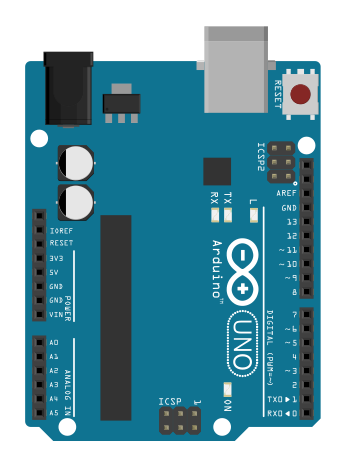
\includegraphics[width=\textwidth]{schnittstellen}};
  % grid
  %\draw[help lines, thick, color=red!90] (0,0) grid (12,16); 
  %\draw[help lines,step=.5] (0,0) grid (12,16);
  %\foreach \x in {0,1,...,12} \node[anchor=north] at (\x,0) {\x};
  %\foreach \y in {0,1,...,16} \node[anchor=east] at (0,\y) {\y};  
  \node[anchor=south west,rounded corners=3pt, draw, color=red!80,line width=3.2pt,text height=1.2cm,text width=2.1cm] (box) at (9,1.5) {};
  \node[below left=0.4cm and -2.4cm of box, color=red!80] {\Huge serielle PINs};
\end{tikzpicture}


\end{document}